\input format.tex

\usepackage{graphicx}
\graphicspath{{cores/}}

\begin{document}

\vspace*{10mm}

\begin{center}
\fontsize{14pt}{16pt}\selectfont\color{black70}{\bf {常道康\textsuperscript{\xiaowuhao{TM}}肠道健康保护力检测报告}}
\end{center}

%% 各章节
\setlength{\arrayrulewidth}{1pt}
\fontsize{8pt}{11pt}\selectfont
\color{gray2}

\begin{LRaside}[.6]{\bf 肠道健康保护力检测说明}
\noindent
\begin{center}

\includegraphics[scale=1.0]{baohulidoctor.pdf}
\end{center}
\asidebreak %
\linespread{1.5}\selectfont {肠道健康是人体健康的重要指征,通过检测肠道中有益菌含量和水平,可以知晓人体肠道健康状况。肠道内有益菌的含量反映了肠道菌群对肠道健康的保护能力,有益菌含量高时,能产生有益物质,抑制有害菌生长,有益于人体健康长寿。有益菌含量低时,有害菌容易过度生长并产生有害物质,危害人体健康。本产品通过检测肠道内常见的四类有益菌:即乳杆菌、双歧杆菌、栖粪杆菌以及阿克曼氏菌,分析您的肠道健康保护力及各类有益菌的含量,及时了解您的肠道微生态平衡及健康状况,并提供定制化的健康管理方案,从而帮助您提高肠道健康保护力,拥有健康肠道,畅享健康生活。}
\end{LRaside}

\vspace*{8mm}

\begin{LRaside2}{\bf 肠道健康保护力评估总分}
\colorbox{topcolor}{\parbox[t]{0.3\textwidth}{
\begin{center}
\textcolor{white}{
\\您的肠道健康保护力评估总分\\
(满分100分)\\
\vspace{6pt}
{\fontsize{15pt}{15pt}\selectfont\bf 15.13分\\}
\vspace{6pt}
肠道保护力优秀,有助于增强免疫力,维护肠道健康
}
\end{center}
}}
\hspace*{6mm}
\colorbox{white}{\parbox[t]{0.62\textwidth}{
\linespread{1.5}\selectfont {
肠道健康保护力评估总分是通过综合评估您肠道内的多种有益菌的含量而得出的一个总的评估指标。有益菌是人类的好朋友,是肠道健康的守护神,能够产生维生素、短链脂肪酸等许多对人体有益的物质,还能抑制有害菌的生长,减少疾病的发生。因此,肠道内有益菌的含量越高,肠道健康保护力评估总分分值也就越高,说明您的肠道健康保护力越强,这将有利于肠道微生态平衡、增强免疫力、促进营养吸收等,从而保证人体健康。\\}}
}
\asidebreak
\bf {指标范围 \vspace*{4mm}\\}
%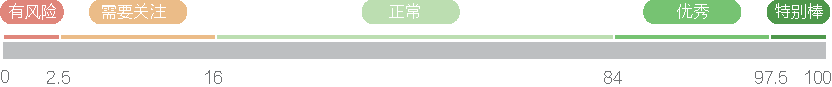
\includegraphics[width=\textwidth]{baohulibar.pdf}
%
\includegraphics[width=\textwidth]{baohulibar02.pdf}

\includegraphics[width=\textwidth]{baohulibar03.pdf}
\end{LRaside2}

\end{document}

